\documentclass[11pt]{article}

\usepackage{fancyhdr}
\usepackage{hyperref}
\usepackage{graphicx}
\usepackage{enumerate}
\usepackage[greek,dutch]{babel} 
\usepackage{listings}
\usepackage{color}
\usepackage{framed}
\usepackage{subfig}

\usepackage[applemac]{inputenc}
\usepackage[T1]{fontenc}
\usepackage[section]{placeins}

\pagestyle{fancy}


\definecolor{mygreen}{rgb}{0,0.6,0}
\definecolor{mygray}{rgb}{0.5,0.5,0.5}
\definecolor{mymauve}{rgb}{0.58,0,0.82}

\lstset{ %
  backgroundcolor=\color{white},         % size of fonts used for the code
  breaklines=true,                 % automatic line breaking only at whitespace
  captionpos=b,                    % sets the caption-position to bottom
  commentstyle=\color{mygreen},    % comment style
  escapeinside={\%*}{*)},          % if you want to add LaTeX within your code
  keywordstyle=\color{blue},       % keyword style
  stringstyle=\color{mymauve},     % string literal style
}



\interfootnotelinepenalty=10000


\title{Raport Project Databases April}
\author{Mathias Beke, Bruno Van de Velde, Elias Van Langenhove, Alexander Vanhulle, Timo Truyts}

\author{
  Mathias Beke
  \and
  Bruno Van de Velde
  \and
  Elias Van Langenhove
  \and
  Alexander Vanhulle
  \and
  Timo Truyts
}


\date{\today}


\setlength{\parindent}{0cm}

\begin{document}

\lhead{Raport Project Databases: April}
\rhead{}



\maketitle


\tableofcontents





\section{Status}




\subsection{Taakverdeling}


\begin{enumerate}
    
   \item \emph{Google/Facebook/OpenID login systeem} Bruno
   
   \item \emph{Wikipedia info toevoegen} Elias
   
   \item \emph{Foto's / Video's van spelers, teams, ...} Elias
   
   \item \emph{User groups} Alexander
   
   \item \emph{Scores van bets, verwerken van weddenschappen} Alexander
   
   \item \emph{Parser} Mathias (en Timo)
   
   \item \emph {Range-based graphs} Timo
   
   \item \emph{Enkele functies toevoegen aan groepen: Invites intrekken, groepen verwijderen, tonen van de bets van alle leden} Alexander
      
   \item \emph{Wikipedia afwerken} Elias
   
   \item \emph{Wikipedia toevoegen aan het geheel} Mathias
   
   \item \emph{Grafieken afwerken} Timo 
   
   \item \emph{Parser afwerken} Timo en Mathias        
   
   \item \emph{Chatbox} Mathias en Alexander
    
   \item \emph{Login vervolledigen} Bruno   
    
\end{enumerate}




\section{Design}


\subsection{UML diagram}

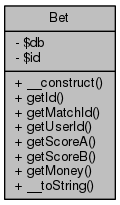
\includegraphics[scale=0.4]{UML_Bet.png}
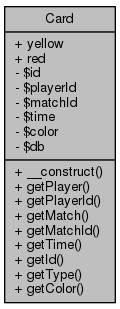
\includegraphics[scale=0.4]{UML_Card.png}
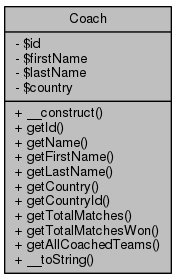
\includegraphics[scale=0.4]{UML_Coach.png}
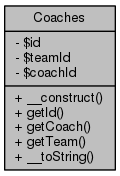
\includegraphics[scale=0.4]{UML_Coaches.png}
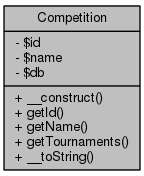
\includegraphics[scale=0.4]{UML_Competition.png}
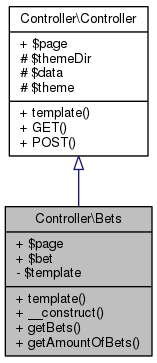
\includegraphics[scale=0.4]{UML_Controller_1_1Bets.png}
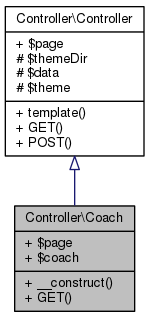
\includegraphics[scale=0.4]{UML_Controller_1_1Coach.png}
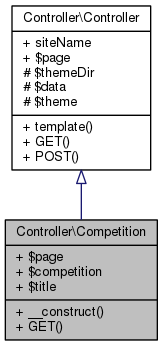
\includegraphics[scale=0.4]{UML_Controller_1_1Competition.png}
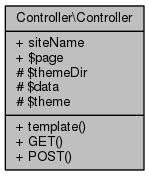
\includegraphics[scale=0.4]{UML_Controller_1_1Controller.png}
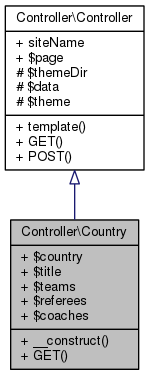
\includegraphics[scale=0.4]{UML_Controller_1_1Country.png}
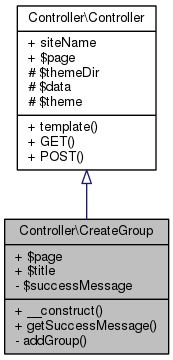
\includegraphics[scale=0.4]{UML_Controller_1_1CreateGroup.png}
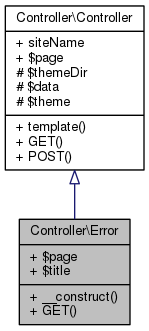
\includegraphics[scale=0.4]{UML_Controller_1_1Error.png}
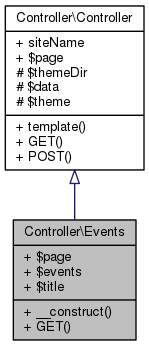
\includegraphics[scale=0.4]{UML_Controller_1_1Events.png}
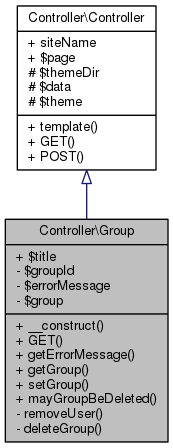
\includegraphics[scale=0.4]{UML_Controller_1_1Group.png}
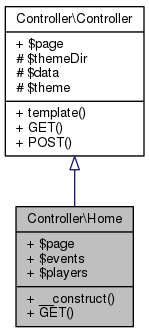
\includegraphics[scale=0.4]{UML_Controller_1_1Home.png}
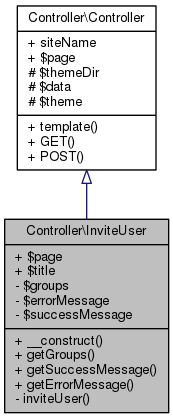
\includegraphics[scale=0.4]{UML_Controller_1_1InviteUser.png}
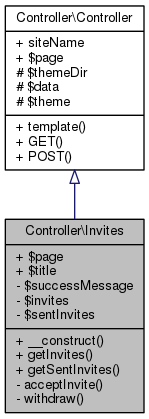
\includegraphics[scale=0.4]{UML_Controller_1_1Invites.png}
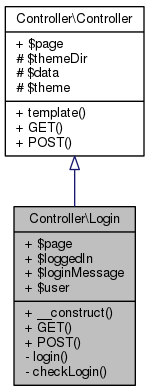
\includegraphics[scale=0.4]{UML_Controller_1_1Login.png}
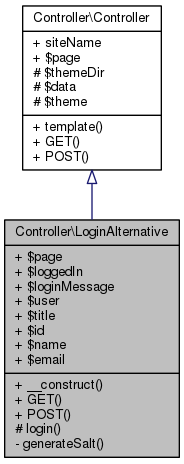
\includegraphics[scale=0.4]{UML_Controller_1_1LoginAlternative.png}
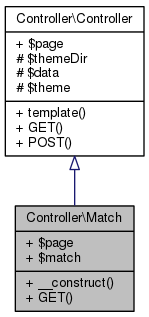
\includegraphics[scale=0.4]{UML_Controller_1_1Match.png}
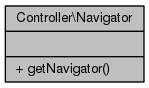
\includegraphics[scale=0.4]{UML_Controller_1_1Navigator.png}
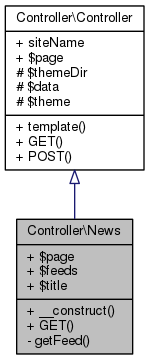
\includegraphics[scale=0.4]{UML_Controller_1_1News.png}
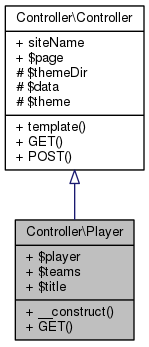
\includegraphics[scale=0.4]{UML_Controller_1_1Player.png}
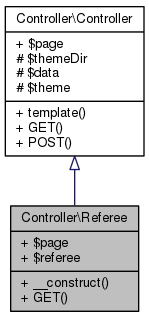
\includegraphics[scale=0.4]{UML_Controller_1_1Referee.png}
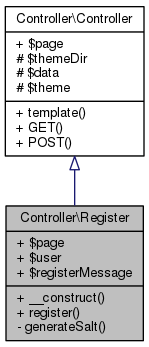
\includegraphics[scale=0.4]{UML_Controller_1_1Register.png}
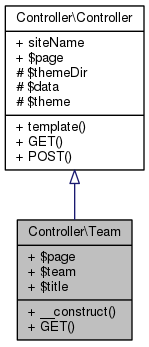
\includegraphics[scale=0.4]{UML_Controller_1_1Team.png}
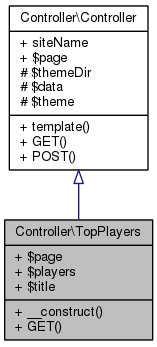
\includegraphics[scale=0.4]{UML_Controller_1_1TopPlayers.png}
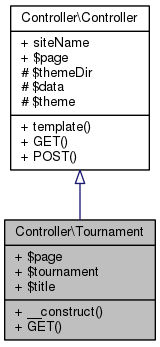
\includegraphics[scale=0.4]{UML_Controller_1_1Tournament.png}
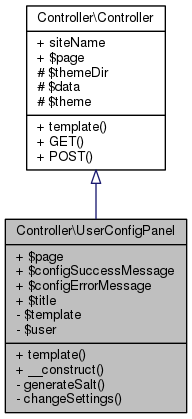
\includegraphics[scale=0.4]{UML_Controller_1_1UserConfigPanel.png}
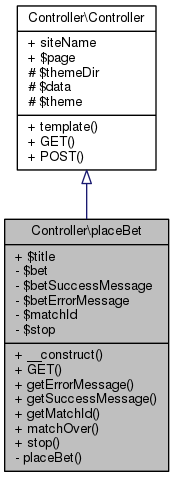
\includegraphics[scale=0.4]{UML_Controller_1_1placeBet.png}
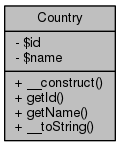
\includegraphics[scale=0.4]{UML_Country.png}
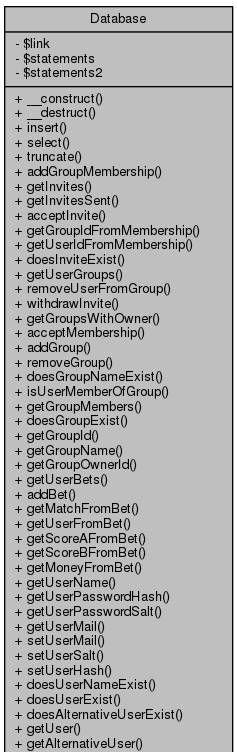
\includegraphics[scale=0.4]{UML_Database1.png}
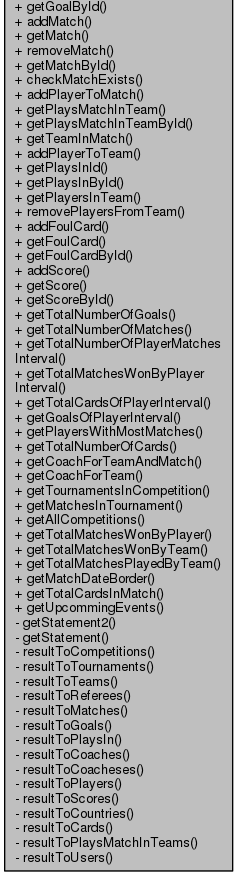
\includegraphics[scale=0.4]{UML_Database2.png}
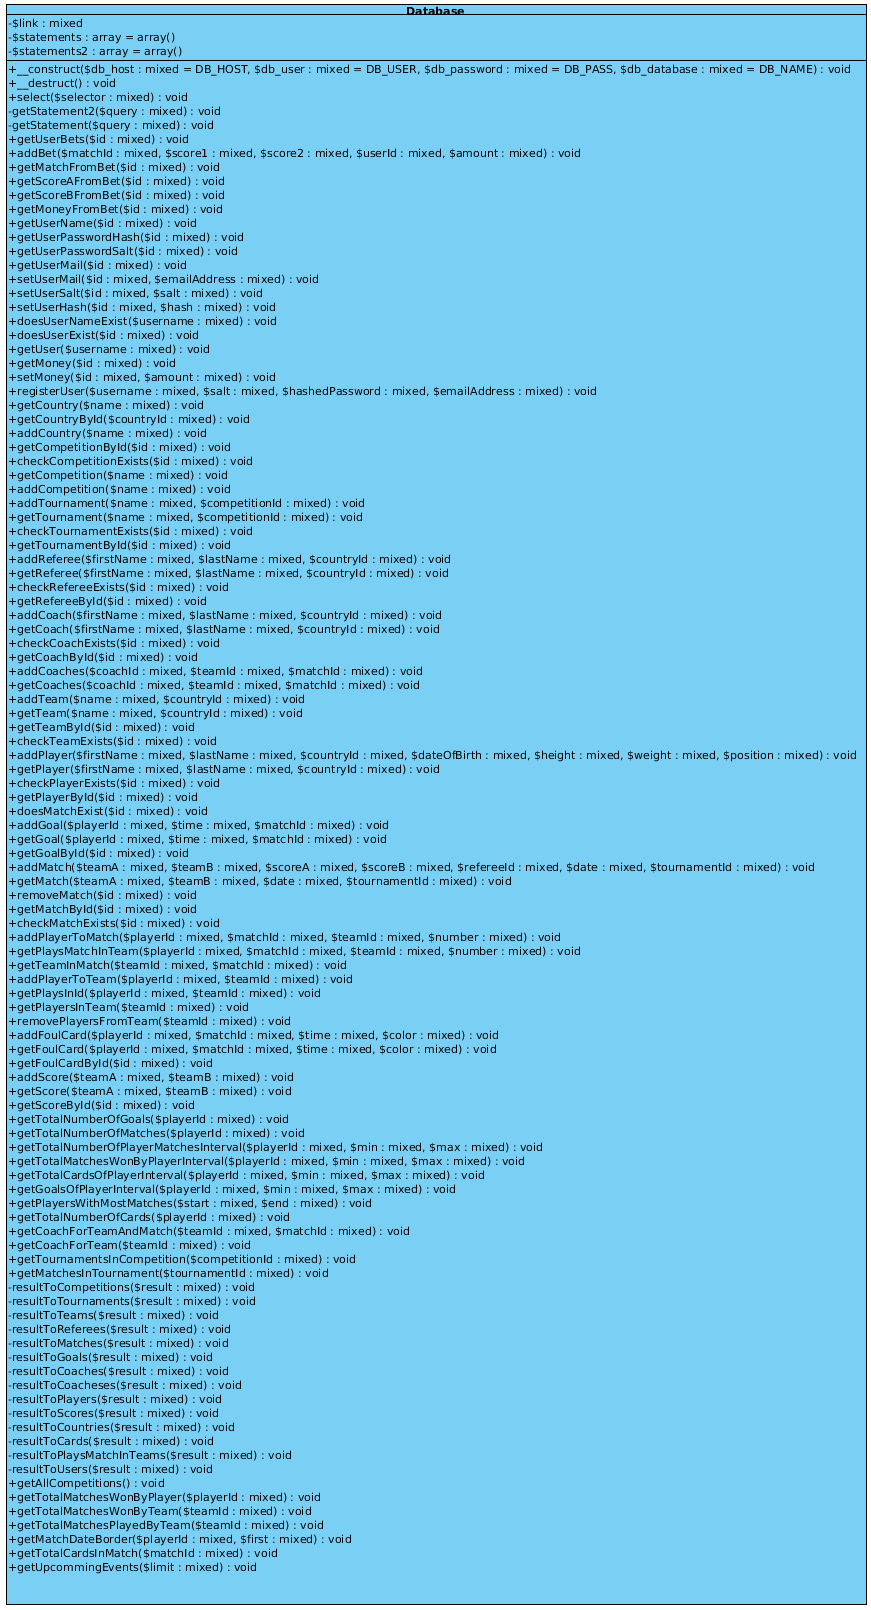
\includegraphics[scale=0.4]{UML_Database3.png}
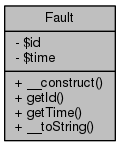
\includegraphics[scale=0.4]{UML_Fault.png}
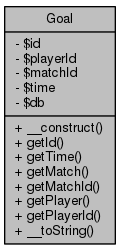
\includegraphics[scale=0.4]{UML_Goal.png}
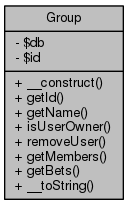
\includegraphics[scale=0.4]{UML_Group.png}
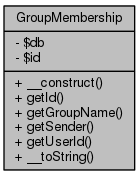
\includegraphics[scale=0.4]{UML_GroupMembership.png}
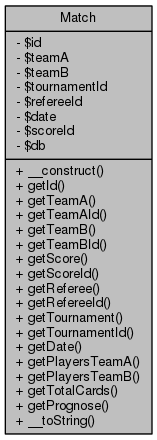
\includegraphics[scale=0.4]{UML_Match.png}
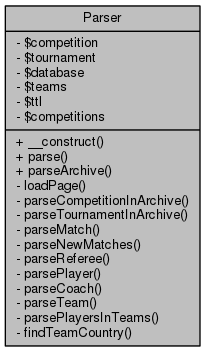
\includegraphics[scale=0.4]{UML_Parser.png}
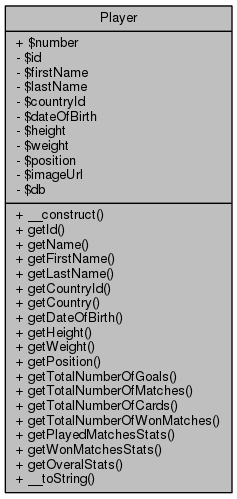
\includegraphics[scale=0.4]{UML_Player.png}
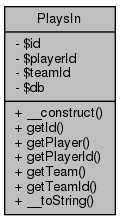
\includegraphics[scale=0.4]{UML_PlaysIn.png}
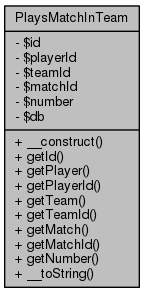
\includegraphics[scale=0.4]{UML_PlaysMatchInTeam.png}
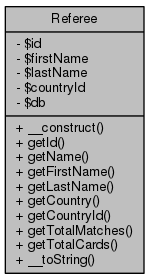
\includegraphics[scale=0.4]{UML_Referee.png}
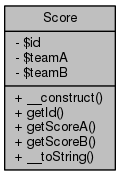
\includegraphics[scale=0.4]{UML_Score.png}
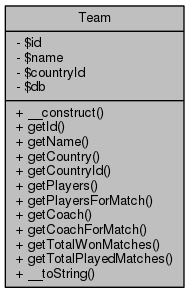
\includegraphics[scale=0.4]{UML_Team.png}
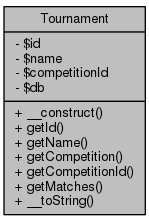
\includegraphics[scale=0.4]{UML_Tournament.png}
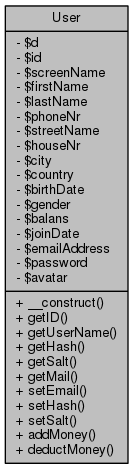
\includegraphics[scale=0.4]{UML_User.png}

\subsection{API}

Om het mogelijk te maken om via javascript interactief informatie van de server
op te halen zijn we begonnen met een api te schrijven.

De api zal antwoorden met json en kan dan eenvoudig in javascript worden gebruikt.

Hier enkele voorbeelden van hoe de api werkt:
\begin{framed}
\begin{lstlisting}
// Returned informatie over alle spelers
/api/player	

// Returned informatie over speler met id 5
/api/player?id=5 

// Returned informatie over alle spelers met voornaam Ronaldo
/api/player?firstname =ronaldo 

// Returned informatie over alle spelers gesorteerd op het aantal gespeelde matchen
/api/player?sort=match
... 
\end{lstlisting}
\end{framed}


\subsection{Parser (GO)}

Bij de aanvang van het project zijn we meteen begonnen met onze parser. We schreven die toen in \emph{PHP} en maakten gebruik van de \emph{PHP Simple HTML DOM Parser}\footnote{\url{http://simplehtmldom.sourceforge.net}}.
Dit framework bleek zeer traag te zijn, en had geheugenlekken. Ook is PHP niet de snelste taal om zulke dingen te doen.\\

Daarom hebben we besloten op de parser opnieuw te beginnen. Ditmaal hebben we deze in \emph{GO} geschreven. \emph{GO} is een programmeertaal die uitermate geschikt is om concurrent te werken. Recent bedacht, maakt de taal concurrent programmeren veel gemakkelijker. Hierdoor wordt \emph{GO} vaak op servers gebruikt.\\

De nieuwe versie van de parser is dus in \emph{GO} geschreven en draait vele malen sneller doordat de competities en tournaments concurrent kunnen geparsed worden. De nieuwe parser zal dit archief dan exporteren in een \emph{JSON} bestand, welk we in PHP importeren en toevoegen aan de database. (Door met een import/export file te werken, moesten we de database toegang niet herschrijven, en konden we de PHP herbruiken.)

Waar PHP er uren over doet, handelt GO de klus af binnen het half uur af. Een geslaagde verbetering dus. 




\section{Database}

\subsection{Schema (ERM-diagram)}

De ERM uit onze vorige versie was reeds redelijk compleet waardoor we hier slechts enkele kleine zaken voor nieuwe functionaliteiten dienden toe te voegen.\\
Hier ging het om de gebruiker-gerelateerde features: het groepen-systeem waardoor een gebruiker lid kan zijn van 0 of meer groepen en het alternatief login systeem waardoor o.a. Google en Facebook accounts nu tevens gebruikt kunnen worden voor het inloggen.  \emph{Zoals vorige keer voegen we de ERM eveneens toe als bijlage zodat deze apart geopend kan worden (zie bijlages/ERM2.png).}

\begin{figure}[h!]
	\begin{center}
	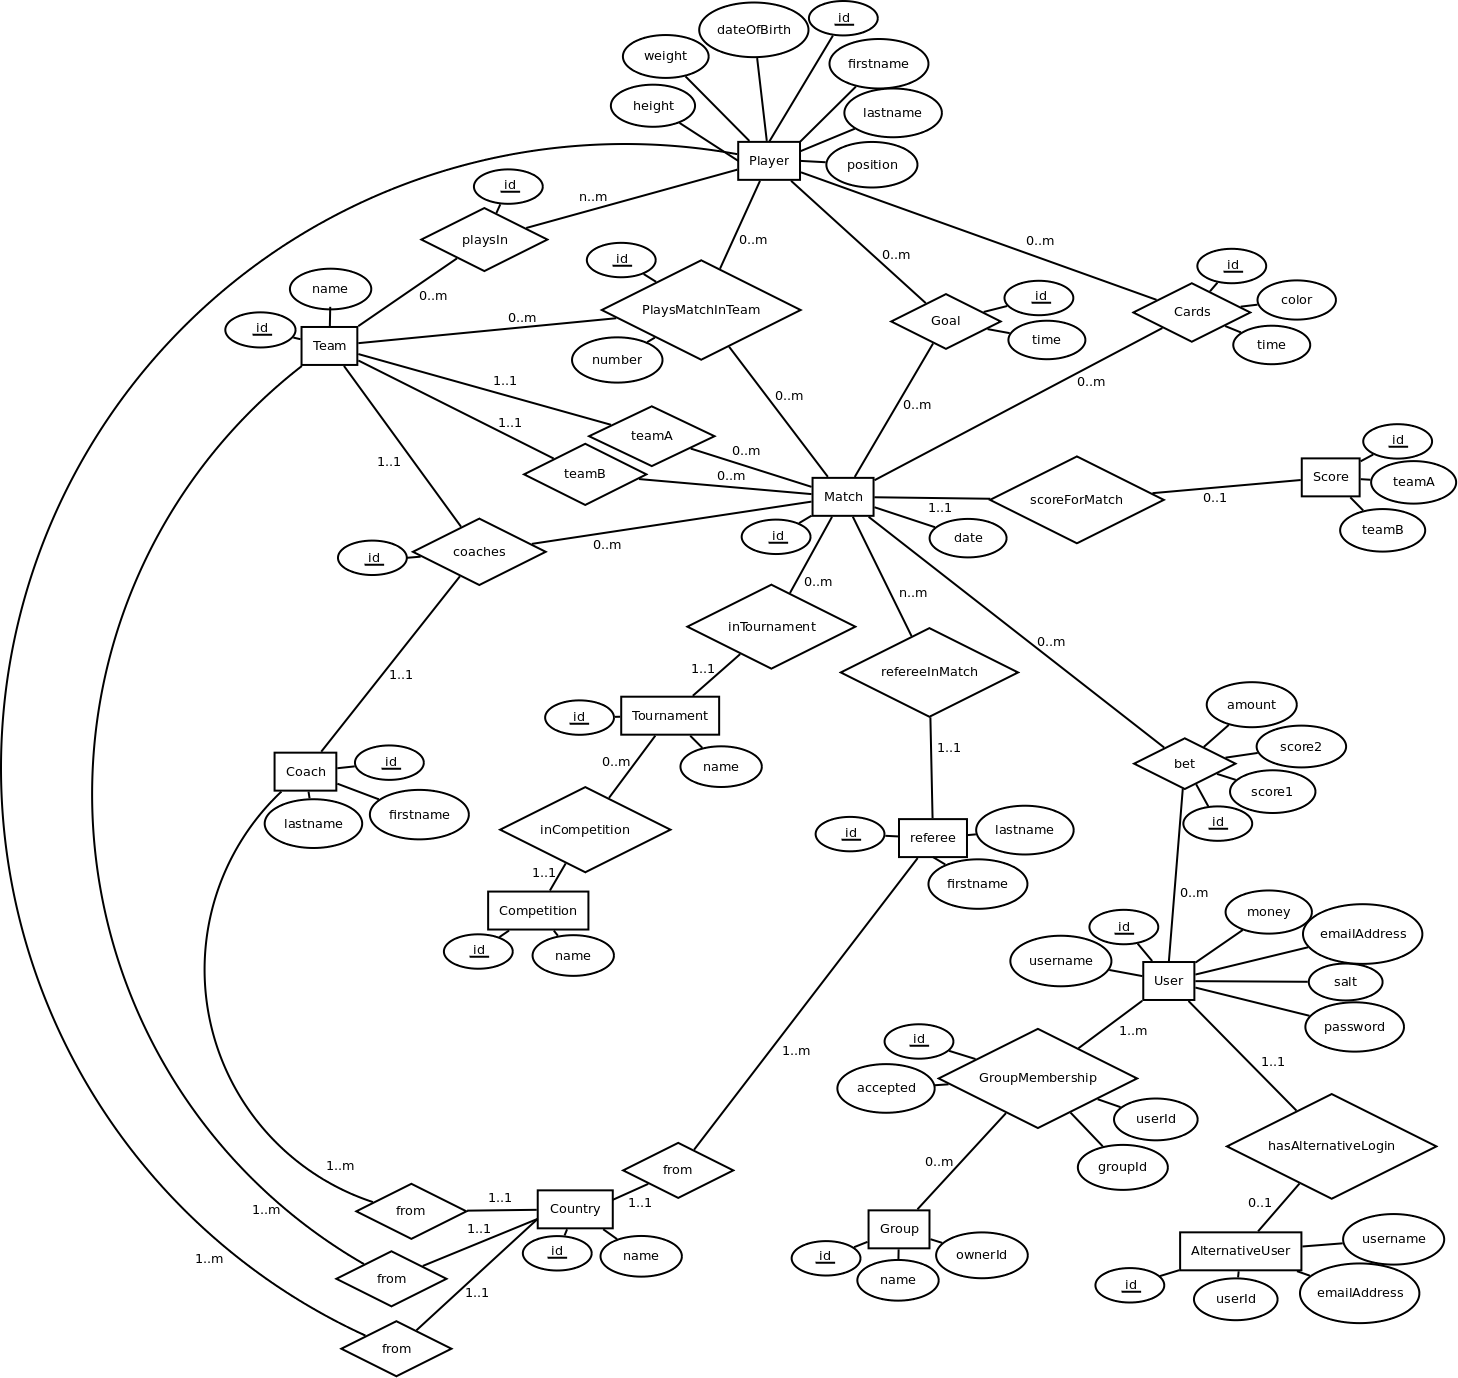
\includegraphics[scale=0.11]{ERM2.png}

	\caption{ERM schema}
	\label{fig:speler}
	\end{center}
\end{figure}
\section{User Interface}


\subsection{Grafieken}

De framework die we gebruikten bleek niet geavanceerd genoeg om bijvoorbeeld te zoomen, ranges te selecteren, etc.\\
We hebben al veel frameworks geprobeerd maar hebben er nog geen gevonden die volledig voldoet aan onze behoeften.\\
Het huidige framework is \emph{jqPlot}\footnote{\url{http://www.jqplot.com}} waarmee we kunnen inzoomen en selecteren welke informatie er getoond moet worden.



\subsection{Gebruikersgroepen}

Een heel gebruikersgroepen systeem werd toegevoegd.  Dit systeem stelt de gebruiker in staat zelf groepen aan te maken, andere gebruikers uit te nodigen enzovoort.  Hieronder een overzicht:\\

Gebruikers kunnen zelf groepen aanmaken.  Hierdoor worden zij de administrator van deze groep en hebben ze volledige rechten.\\

\begin{figure}[h!]
	\begin{center}
	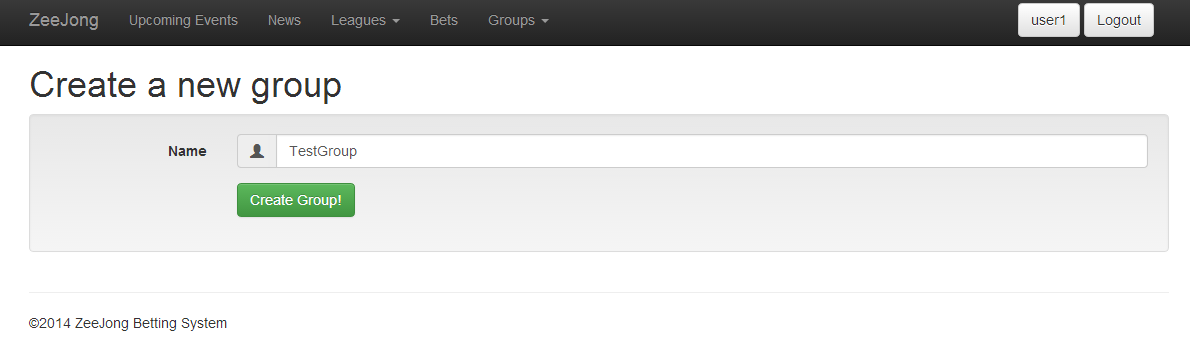
\includegraphics[scale=0.4]{createGroup.png}

	\caption{Create Group}
	\label{fig:createGroup}
	\end{center}
\end{figure}

Nadat de groep aangemaakt is, kan de beheerder andere gebruikers uitnodigen.  Hiervoor is een formulier met een drop-down menu voorzien om tussen de verschillende groepen te kiezen waarvan de gebruiker administrator is.\\

\begin{figure}[h!]
	\begin{center}
	\includegraphics[scale=0.4]{inviteUser.png}

	\caption{Invite User}
	\label{fig:inviteUser}
	\end{center}
\end{figure}

Elke gebruiker heeft een venster waarop de uitnodigingen zichtbaar zijn die deze gebruiker ontvangen heeft en die de gebruiker verstuurd heeft.  Een uitnodiging kan geaccepteerd/ingetrokken worden.\\

\begin{figure}[h!]
	\begin{center}
	\includegraphics[scale=0.4]{invites.png}

	\caption{Invites}
	\label{fig:invites}
	\end{center}
\end{figure}

Wanneer een gebruiker een uitnodiging aanvaard heeft, wordt de groep toegevoegd aan het drop-down menu in de header waardoor de gebruiker naar de groep kan navigeren.\\

\begin{figure}[h!]
	\begin{center}
	\includegraphics[scale=0.4]{inviteAccepted.png}

	\caption{Invite Accepted}
	\label{fig:inviteAccepted}
	\end{center}
\end{figure}

In het groepsvenster kan de gebruiker bets van andere spelers van de groep zien.  Een gebruiker kan ook uit de groep vertrekken.  Indien de gebruiker tevens de administrator is, dan kan hij andere gebruikers uit de groep verwijderen en eventueel de groep zelf opdoeken.\\

\begin{figure}[h!]
	\begin{center}
	\includegraphics[scale=0.4]{group.png}

	\caption{Group}
	\label{fig:group}
	\end{center}
\end{figure}

\section{User Interface}





\section{Extra Functionaliteit}


\subsection{Wiki}

Nu wordt op de speler pagina ook de introductie van de speler op wikipedia getoond.
Deze pagina wordt gevonden door eerst te zoeken naar een sectie met als naam de naam van de speler.
Indien deze niet gevonden kan worden wordt er een \emph{Wikipedia} search gedaan met als termen de volledige naam van de speler en wordt zo de speler pagina gevonden.
Voor het laden van deze tekst wordt \emph{wikidrain}\footnote{\url{https://github.com/abreksa4/wikidrain}} gebruikt, mits enige aanpassingen die we zelf toegepast hebben.


\subsection{RSS nieuwsfeed}

De RSS nieuwspagina werd uitgebreid met extra feeds. De gebruiker krijgt bovenaan een menuutje, waarin hij een feed kan uitkiezen om het nieuws te lezen.
De urls naar de feeds worden bijgehouden in een JSON file, zodat het toevoegen van extra feeds amper werk is.

Intern werkt de RSS nog steeds met \emph{SimplePie}\footnote{url{http://simplepie.org}} rss parser.



\subsection{OpenID}

Naast de normale login is er ook een optie om in te loggen door gebruik te maken van een externe account. Wanneer je naar de alternatieve login pagina gaat, krijg je een keuze uit verschillende services (zoals \emph{Facebook} en \emph{Google}) waarmee je kunt inloggen. Buiten Facebook werken deze allen met \emph{OpenID} en er is uiteindelijk voor de \emph{LightOpenID}\footnote{\url{https://code.google.com/p/lightopenid/}} library gekozen omdat deze makkelijk te gebruiken was. \emph{Facebook} is achteraf nog apart toegevoegd aangezien die helemaal geen \emph{OpenID} provider is. Om in te kunnen loggen via \emph{Facebook} moest eerst een app worden aangemaakt op hun site om alles mogelijk te maken. Buiten het feit dat er extra code nodig is die het verschil tussen een \emph{OpenID} en een \emph{Facebook} login checked, is het grote nadeel dat de \emph{Facebook} login enkel op de server kan werken en niet ondertussen op de localhost getest kan worden. Maar dit heeft geen gevolgen voor de gebruikers van de site.




\section{Planning}


De verdere planning focust zich vooral op kleine verbeteringen.
We hopen dat we geen structurele veranderingen meer moeten doorvoeren.



\section{Appendix}

\subsection{Queries}

\paragraph{Accepteren van invite}

  Deze query past de groepslidmaatschappen van de user aan door een nieuwe groep toe te voegen.

  \begin{framed}
  \begin{lstlisting}[language=sql]
UPDATE GroupMembership
SET accepted = ?
[WHERE id = ?];
  \end{lstlisting}
  \end{framed}

\paragraph{User verwijderen uit groep}

  Deze query verwijdert een gegeven user uit een gegeven groep.

  \begin{framed}
  \begin{lstlisting}[language=sql]
DELETE 
FROM `GroupMembership` 
[WHERE id = ? AND 
groupId = ?];
  \end{lstlisting}
  \end{framed}
  
\paragraph{groep verwijderen}

  Deze query verwijdert een gegeven groep.

  \begin{framed}
  \begin{lstlisting}[language=sql]
DELETE 
FROM `Group` 
[WHERE id = ?];
  \end{lstlisting}
  \end{framed}  
  
\paragraph{Invite intrekken}

  Deze query trekt een gegeven verzonden invite weer in.

  \begin{framed}
  \begin{lstlisting}[language=sql]
DELETE 
FROM `GroupMembership` 
[WHERE id = ? AND 
accepted = False];
  \end{lstlisting}
  \end{framed}
  
\paragraph{Invite accepteren}

  Deze query accepteert een invite van een gegeven user voor een gegeven groep.

  \begin{framed}
  \begin{lstlisting}[language=sql]
UPDATE `GroupMembership`
SET accepted = True
[WHERE id = ? AND 
groupId = ?];
  \end{lstlisting}
  \end{framed}  

\paragraph{Uitnodigen verzonden door gebruiker}

  Deze query vraagt de uitnodigingen op die verzonden zijn door een gegeven user.

  \begin{framed}
  \begin{lstlisting}[language=sql]
SELECT GroupMembership.id
  FROM GroupMembership
  [INNER JOIN `Group` ON 
  GroupMembership.groupId=Group.id]
  [WHERE Group.ownerId=? AND
   GroupMembership.accepted=0]
  \end{lstlisting}
  \end{framed}


\paragraph{Gewonnen wedstrijden van speler binnen interval}

  Deze query vraagt de hoeveelheid matches waarbij de gegeven speler voor het winnende team speelde binnen een gegeven tijdspanne op.

  \begin{framed}
  \begin{lstlisting}[language=sql]
SELECT COUNT(*)
 FROM `PlaysMatchInTeam`
 [JOIN `Match` ON `Match`.id = matchId]
 [JOIN `Score` ON `Score`.id = scoreId]
 [WHERE playerId = ? AND
 `Match`.date > ? AND
 `Match`.date < ? AND
    ((teamId = `Match`.teamA AND `Score`.teamA > `Score`.teamB) OR
    (teamID = `Match`.teamB AND `Score`.teamB > `Score`.teamA))];
  \end{lstlisting}
  \end{framed}



\end{document}
